\documentclass[10pt]{article}
%%%%%%%%%%%%%%%%%%%%%%%%%%%%%%%%%%%%%%%%
\usepackage{amsmath}
\usepackage{verbatim}
\usepackage[usenames,dvipsnames]{color}
\usepackage{ulem}
\usepackage{setspace}
\usepackage{lscape}
\usepackage{longtable}
\usepackage[top=1.25in,bottom=1.5in,left=1in,right=1.5in,landscape]{geometry}
\usepackage{graphicx}
\usepackage{epstopdf}
\usepackage[usenames,dvipsnames]{pstricks}
\usepackage{epsfig}
\usepackage{pstricks-add}
\usepackage{pst-node}
\usepackage{fancyhdr}
\usepackage[absolute,showboxes]{textpos}

%TCIDATA{OutputFilter=LATEX.DLL}
%TCIDATA{Version=5.00.0.2552}
%TCIDATA{<META NAME="SaveForMode" CONTENT="1">}
%TCIDATA{Created=Thursday, August 28, 2003 13:38:44}
%TCIDATA{LastRevised=Thursday, August 14, 2008 15:20:27}
%TCIDATA{<META NAME="GraphicsSave" CONTENT="32">}
%TCIDATA{<META NAME="DocumentShell" CONTENT="Standard LaTeX\Blank - Standard LaTeX Article">}
%TCIDATA{Language=American English}
%TCIDATA{CSTFile=LaTeX article (bright).cst}

\setcounter{MaxMatrixCols}{10}

\newenvironment{proof}[1][Proof]{\noindent\textbf{#1.} }{\ \rule{0.5em}{0.5em}}
\setlength{\columnsep}{.2in}

\renewcommand{\labelitemii}{$\cdot$}

\pagestyle{fancy} \fancyhead{} \fancyfoot{} \rfoot{} \lfoot{}

\newcommand{\slide}[2]{
\begin{textblock}{11}(0,0)
\textcolor{Black}{\textbf{\huge \rule{0pt}{1in} \raisebox{.2in}{#1}}}
\end{textblock}
\begin{Large} \noindent
#2
\end{Large}
\vfill \pagebreak}

\setlength{\TPHorizModule}{1in}
\setlength{\TPVertModule}{1in}
\textblockcolour{Yellow}
\renewcommand{\headrulewidth}{0pt}



\begin{document}
\onehalfspacing 

\lfoot{Math and Terminology} \rfoot{Economic Growth}

\slide{Mechanics}{Simplest growth model is something like
\begin{equation}
y(t) = y_0 e^{gt}
\end{equation}
\begin{itemize}
	\item $y(t)$ is output per worker at time $t$
	\item $y_0$ is output per worker at some initial time $0$
	\item $g$ is the growth rate of output per worker
	\item $e^{gt}$ gives us exponential growth
\end{itemize}

\vspace{.25in}\noindent Simpler to draw/graph/analyze this in log terms, so take
\begin{equation}
\ln y(t) = \ln y_0 + gt.
\end{equation}

}

\slide{Rules for Logs}{I used a few rules for taking logs there. Here are the ones you need to know.
\begin{itemize}
	\item $\ln{XZ} = \ln{X} + \ln{Z}$
	\item $\ln{X/Z} = \ln{X} - \ln{Z}$
	\item $\ln{X^{\alpha}} = \alpha \ln{X}$
	\item $\ln{e^{X}} = X$
\end{itemize}

\vspace{.25in}\noindent ``take logs'' and ``take the natural log'' are synonyms in this class. We are always implicitly using natural logs - the $\ln{X}$ symbol.

\vspace{.25in}\noindent These rules roll up on one another, so
\begin{equation}
\ln{X^{\alpha}Z/W^{\beta}} = \alpha \ln{X} + \ln{Z} - \beta \ln{W}
\end{equation}
}

\slide{Log Output per worker}{Our simple model
\begin{equation}
\ln y(t) = \ln y_0 + gt.
\end{equation}
describes a line. $\ln{y(t)}$ is the y variable, $t$ is the x. 
\begin{itemize}
	\item $y_0$ is the intercept
	\item $g$ is the slope
\end{itemize}
}

\slide{Log Output per worker}{$y(t)$ is roughly linear for lots of advanced countries
\begin{center}
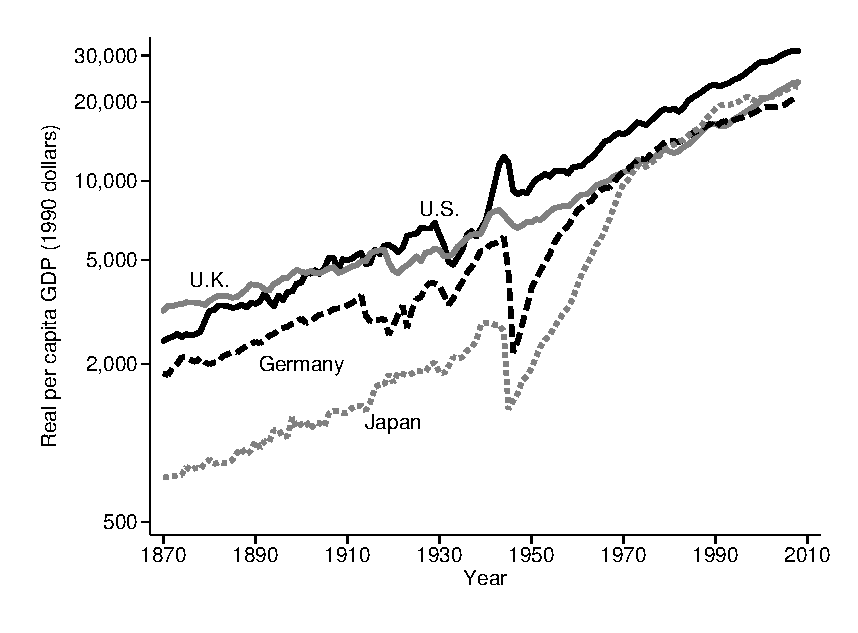
\includegraphics[scale=1.3]{figure_3_3.eps}
\end{center}
}

\slide{Identifying Different Effects}{In terminology, distinguish
\begin{itemize}
	\item \textit{Level Effects}: These are things that shift the intercept, $y_0$, up or down. In the early 1900's Japan was at a distinctly lower \textit{level} than the U.S. or U.K.
	\item \textit{Growth Effects}: These are things that shift the slope, $g$. For the most part, $g$ is constant for all those countries in the diagram.
	\item \textit{Transitional Effects}: This is growth that occurs as a country moves from one level to another. Temporary spurt in growth rate (a very steep line) that catches a country up to some level. See Japan and Germany in the diagram after WWII.
\end{itemize}

\vspace{.25in}\noindent As a preview, here is what we are going to see in the class
\begin{itemize}
	\item The growth rate, $g$, is probably the same across countries, or very close. There are very few examples of true growth effects.
	\item Much of the distinction in observed growth rates between countries is due to transitional growth - China catching up to the West, for example.
	\item Much of the explanation for why some countries are poor and some are rich is due to level effects.
\end{itemize}

}

\slide{Transitional and Level Effects}{Our simple model is too simple to capture transitional effects, which occurs because output per worker doesn't have to be exactly on the line described by $y(t) = y_0 e^{gt}$ . If $y_0$ jumps at some point, then our simple model predicts:
\begin{center}
\scalebox{1.3}{
\begin{pspicture}(10,9)
\psline{->}(0,0)(9,0) \psline{->}(0,0)(0,8) \rput(9.7,0){$Time$} \rput(0,8.3){$\ln{y}$}
\psline(0,1)(3,2) \psline(3,4)(9,6) \psline[linestyle=dotted](3,4)(3,0) \rput(6,3){Big noticeable jump}
\end{pspicture}
}
\end{center}
}

\slide{Transitional and Level Effects}{But we don't see leaps like this in the data. We see
\begin{center}
\scalebox{1.3}{
\begin{pspicture}(10,9)
\psline{->}(0,0)(9,0) \psline{->}(0,0)(0,8) \rput(9.7,0){$Time$} \rput(0,8.3){$\ln{y}$}
\psline(0,1)(3,2) \pscurve(3,2)(5,4)(9,6) \psline[linestyle=dotted](3,4)(3,0) \rput(6.5,3){Smooth transition}
\psline[linestyle=dashed,dash=3pt 2pt](3,4)(9,6)
\end{pspicture}
}

Note that for a while output is not on the line described by our simple model.
\end{center}
}

\slide{Transitional and Level Effects}{The Solow Model we'll start with captures this smooth transition
\begin{itemize}
	\item Output depends on stock of accumulated capital (physical machines, human capital, etc..)
	\item Output cannot ``jump'' to new level even if $y_0$ jumps
	\item Takes time to accumulate capital to reach new level
\end{itemize}

\vspace{.25in}\noindent A level effect (jump in $y_0$) will cause transitional effects - Japan after WWII

\vspace{.25in}\noindent Or, if $y$ falls ``off'' the simple line, we'll get transitional growth - Germany after WWII 
}


\slide{Calculating Growth Rates}{We would typically write
\begin{equation}
\frac{y(t+k) - y(t)}{y(t)}
\end{equation}
to calculate the percent growth rate from period $t$ to period $t+1$. Given our simple model, this is
\begin{equation}
\frac{y(t+1) - y(t)}{y(t)} = \frac{y(t+1)}{y(t)} - 1 = \frac{y_0 e^{g(t+1)}}{y_0 e^{gt}} - 1 = e^{g}-1
\end{equation}

\vspace{.25in}\noindent It is true that $e^{g} \approx 1+g$ for small values of $g$ (like $g<0.05$). So therefore
\begin{equation}
\frac{y(t+1) - y(t)}{y(t)} \approx g
\end{equation}

\vspace{.25in}\noindent Or, take the difference in log output
\begin{equation}
\ln y(t+1) - \ln y(t) = \ln y_0 + g (t+1) - \ln y_0 - gt = g
\end{equation}
So we will typically take the difference in logs to find the growth rate. This is essentially the same as calculating the percent change like we did above.
}

\slide{Logs and Time Derivatives}{We'll be using this a lot. It's a mechanical technique to find out how some function grows over time. In our example, we've got $y(t) = y_0 e^{gt}$. We've already taken logs
\begin{equation}
\ln y(t) = \ln y_0 + gt
\end{equation}
and now we need to take the time derivative
\begin{equation}
\frac{\partial \ln y(t)}{\partial t} = \frac{\partial \ln y_0}{\partial t} + \frac{\partial gt}{\partial t}
\end{equation}
and this is
\begin{equation}
\frac{\partial y(t)\partial t}{y(t)} = g
\end{equation}
where I've assumed that $y_0$ is constant over time. 

\vspace{.25in}\noindent For notational convenience, write
\begin{equation}
\frac{\partial y(t)/\partial t}{y(t)} = \frac{\dot{y}}{y} = g
\end{equation}
where the $\dot{y}$ just means the change in $y$ over time. 

\vspace{.25in}\noindent Note that ``take logs and derivatives'' is really just like looking at a percent change (difference in $y$ over $y$). 
}

\slide{Logs and Time Derivatives}{With production functions, we'll be doing all sorts of log-ing and derivative-ing. Take
\begin{equation}
Y = K^{\alpha} X^{\beta} L^{1-\alpha-\beta}
\end{equation}
as an example. Taking logs we get
\begin{equation}
\ln Y = \alpha \ln{K} + \beta \ln{X} + (1-\alpha-\beta)\ln{L}
\end{equation}
using our rules for logs. Then time derivatives are
\begin{equation}
\frac{\dot{Y}}{Y} = \alpha \frac{\dot{K}}{K} + \beta \frac{\dot{X}}{X} + (1-\alpha-\beta) \frac{\dot{L}}{L} 
\end{equation}

\vspace{.25in}\noindent This tells us that the growth rate on the left (of $Y$) is equal to a sum of the growth rates of the things on the right.
}

\slide{Steady State}{A \textit{steady state} is a situation in which a dynamic variable stops changing. That is, perhaps we have some variable $K$ described by
\begin{equation}
\dot{K} = sK^{\alpha} - \delta K
\end{equation}
which could also be divided by $K$ to show things in terms of growth rates
\begin{equation}
\frac{\dot{K}}{K} = sK^{\alpha-1} - \delta.
\end{equation}

\vspace{.25in}\noindent Regardless, where will $K$ have a steady state? That is, at what value of $K$ will $K$ stop changing? $\dot{K}$ measures the change in $K$, so it is where $\dot{K} = 0$, or where
\begin{equation}
s K^{\alpha} = \delta K
\end{equation}
which implies that
\begin{equation}
K^{\ast} = \left( \frac{s}{\delta}  \right)^{1/(1-\alpha)}
\end{equation}
where $K^{\ast}$ is used to denote this steady state. If $K = K^{ast}$, then $K$ will not change, and therefore will remain \textit{steady} at the value $K^{\ast}$ forever.
}

\slide{Real GDP Comparisons}{We talk about $y(t)$ as output per worker. How do we measure that? In particular, how do we compare that across countries, who use different currencies and have different relative prices?
\begin{itemize}
	\item Convert GDP in each country to common currency (dollar or ``international dollar'') using exchange rates
	\item Find real output of each ``good'' by dividing domestic expenditure by domestic price
	\item Calculate ``Real GDP'' by valuing real output of each good at a given international price
\end{itemize}

\vspace{.25in}\noindent Example. India spends \$3,000 per capita on food and \$1,000 per capita on cell phones. Indian prices are \$2 per unit of food and \$10 per phone. Intl. price is \$3 per unit of food and \$5 per phone
\begin{itemize}
	\item Domestic GDP is $3000 + 1000 = 4000$.
	\item Real output is 3000/2 = 1500 units of food and 1000/10 = 100 units of cell phones.
	\item Real GDP is $1500\times3 + 100\times5 = 5000$
\end{itemize}

}

\slide{Real GDP Comparisons}{The set of prices we use to value goods matter a lot in international comparisons. 
\begin{itemize}
	\item International Comparison of Prices project collects prices for goods/services across the globe
	\item Comes up with ``common price'' for each good - but this is weighted heavily towards rich countries
	\item So real GDP measures we use in class value each country's output at rich country prices
	\item This can have distorting effects - in general it makes poor countries look relatively well off
	\item Why? Because the common price is high for things that poor countries have a lot of (services) but low for things that poor countries have little of (high-tech goods)
\end{itemize}

\vspace{.25in}\noindent There is no ``right'' set of prices to use to compare countries. But you have to pick one set of prices to use for comparison. 
}


\end{document}